% -*- coding: utf-8 -*-
% !TEX encoding = UTF-8 Unicode
% !TEX root =  main.tex

\chapter{Theoretische Grundlagen und begriffliche Erklärungen}\label{cha:grundlagen}

Um auf die Regelung einer anisotropen Synchronmaschine einzugehen, werden im folgenden einige Grundlagen erörtert.

\section{Dreiphasensystem}\label{sec:dreiphasensystem}

\begin{figure}[h]
\centering
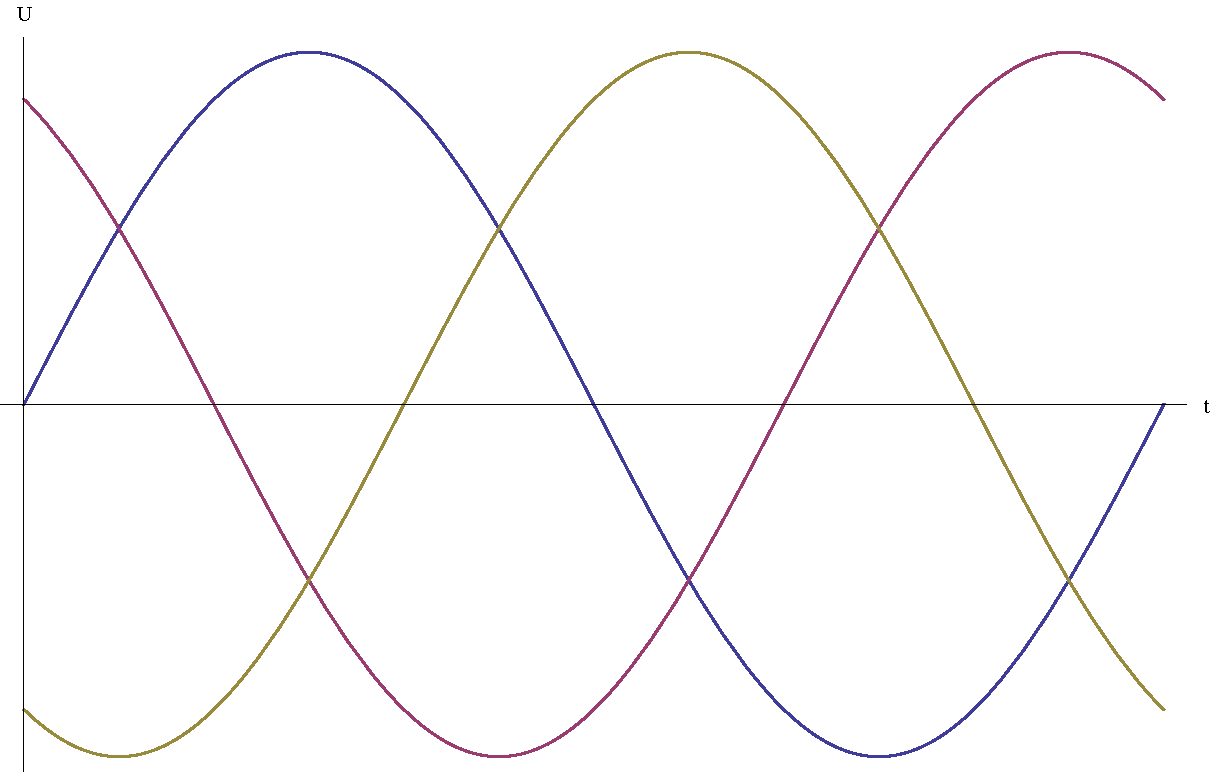
\includegraphics[width=0.5\textwidth]{dreiphasensystem.pdf}
\label{fig:dreiphasensystem}
\caption{Darstellung des Dreiphasensystem mit \textsc{Mathematica}.}
\end{figure}

\section{Einführung Magnetfelder}\label{sec:magnetfelder}

\subsection{Strombelag}\label{sec:strombelag}

Die zeitliche und örtliche Änderung von Magnetfeldern in elektrischen Maschinen wird bestimmt durch die Anordnung stromdurchflossener Leiter und die Art der Speisung \parencite[S.~199]{hofmann2013}.
Die räumliche Verteilung des Stromes wird durch den Strombelag wiedergegeben.
Wenn die Oberfläche eines ferromagnetischen Körpers einen Strombelag $A$ führt, d.\ h.\ wenn eine flächenhafte Strömung vorliegt, liefert das Durchflutungsgesetz

\begin{align}
\oint_{s}{\vec{H}d\vec{s}} = w\cdot I = \Theta \label{durchflutungsgesetz}
\end{align}

$Hds=Ads$, d.\ h.\ $H = A$ bzw.\ $B = \mu A$.
Folgernd existieren neben den Normalkomponenten, $B_n$ und $H_n$ die Tangentialkomponenten $H_t$ und $B_t$ der Feldgrößen.
Die Feldlinien treten nicht mehr senkrecht aus der Randkurve aus, sondern unter einem Winkel $\alpha$.

\begin{align}
\alpha = \arctan(\frac{B_n}{\mu A}) \label{strombelagwinkel}
\end{align}

Der Strombelag wird über dem Umlauf einer Spule bzw.\ Spulengruppe angegeben.

\begin{align}
\Theta(x) = - \int_{x_0}^{x} A(x)dx \label{durchflutung}
\end{align}

damit erhält man durch Differentation den Strombelag $A$

\begin{align}
A(x) = -\partial_x \Theta(x) \label{Strombelag}
\end{align}

mit

\begin{align}
\Theta(x) = \hat{\Theta}(x)\cdot \cos(\frac{\pi}{\tau_p}(x-x_\mu)) \label{adurchflutung}
\end{align}

Nach \ref{durchflutung} ist offensichtlich, dass eine sinusförmige Durchflutungsverteilung nur dann entstehen kann, wenn der Ankerstrombelag ebenfalls sinusförmig, aber um eine Polteilung versetzt ist \parencite[S.~247]{mullerI2005}.

%\begin{figure}[h]
%\centering
%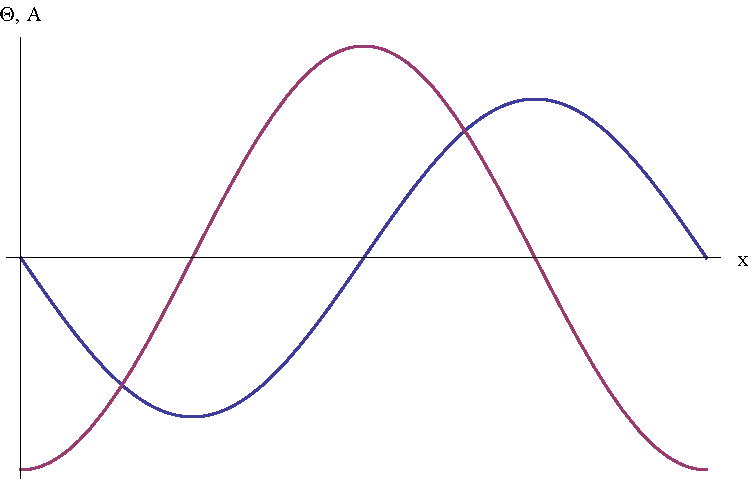
\includegraphics[width=0.5\textwidth]{strombelag.pdf}
%\label{fig:strombelag}
%\caption{Darstellung des sinusförmigen Verlaufs des Strombelags über dem Umlauf.}
%\end{figure}

\subsection{•}

\section{Induktivitäten}\label{sec:induktiv}

\section{Einführung Synchronmaschine}\label{sec:synchron}

\section{Permanenterregte Synchronmaschine}\label{sec:pmsm}

\section{Evalurierung der Ersatzschaltbilder für die Regelung}\label{sec:esb}

%%% Local Variables: 
%%% mode: latex
%%% TeX-master: "main"
%%% TeX-open-quote: "\\enquote{"
%%% TeX-close-quote: "}"
%%% LaTeX-csquotes-open-quote: "\\enquote{"
%%% LaTeX-csquotes-close-quote: "}"
%%% End: 

